% PART 5: Practical Implementation
\chapter{Practical Implementation}
The Project repositories are hosted on GitHub, are public and can be accessed by following these references: Back-end Core Logic\cite{alexei_pavlovschii_blocksign_nodate} and Front-end User Interface\cite{vladimir_vitcovschii_blocksign_nodate}.

\section{Back-end architecture}
The back-end of the system has been developed with a focus on scalability, modularity, and security. Its purpose is to provide all the critical functionality required for user registration, authentication, document management, and secure verification of signatures (Figure \ref{main-project-routers}). 

\begin{figure}[H]
    \centering
    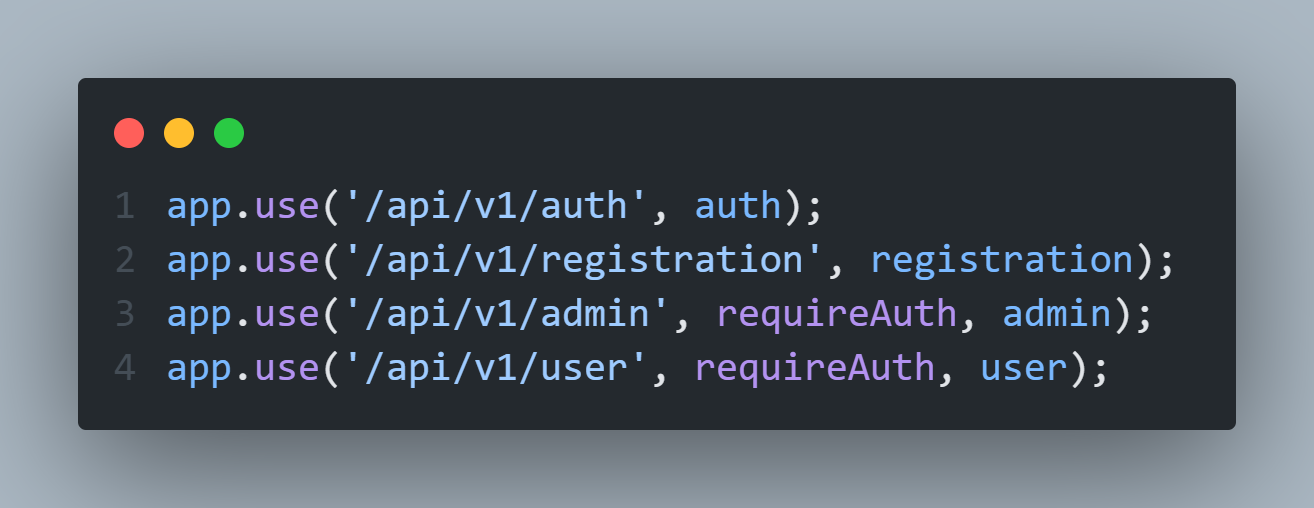
\includegraphics[width=18cm]{"images/main-project-routers.png"}
    \caption{Main Project Routers}
    \label{main-project-routers}
\end{figure}

The implementation relies on Node.js with the Express.js framework, while data persistence is handled by PostgreSQL through the Prisma ORM.

\subsection{Application Layer}
The server is structured around separate route modules, each of which is responsible for a specific part of the functionality. For example, the auth.routes.ts file manages the passwordless login process using challenge–response verification, while registration.routes.ts covers the steps of email OTP verification, registration requests, and account completion with a public key. The administrator’s responsibilities, such as reviewing and approving registration requests, are implemented in admin.registration.routes.ts. Finally, user-oriented functionality, including profile management and document operations, is centralized in user.routes.ts. This modular design improves maintainability and makes it easier to extend the system in the future.

\subsection{Database Layer}
The database schema is implemented using Prisma ORM on top of PostgreSQL. Entities such as User, RegistrationRequest, Document, DocumentParticipant and Signature are modeled explicitly with foreign keys and unique constraints to guarantee consistency (Figure \ref{user-db-model}). 

\begin{figure}[H]
    \centering
    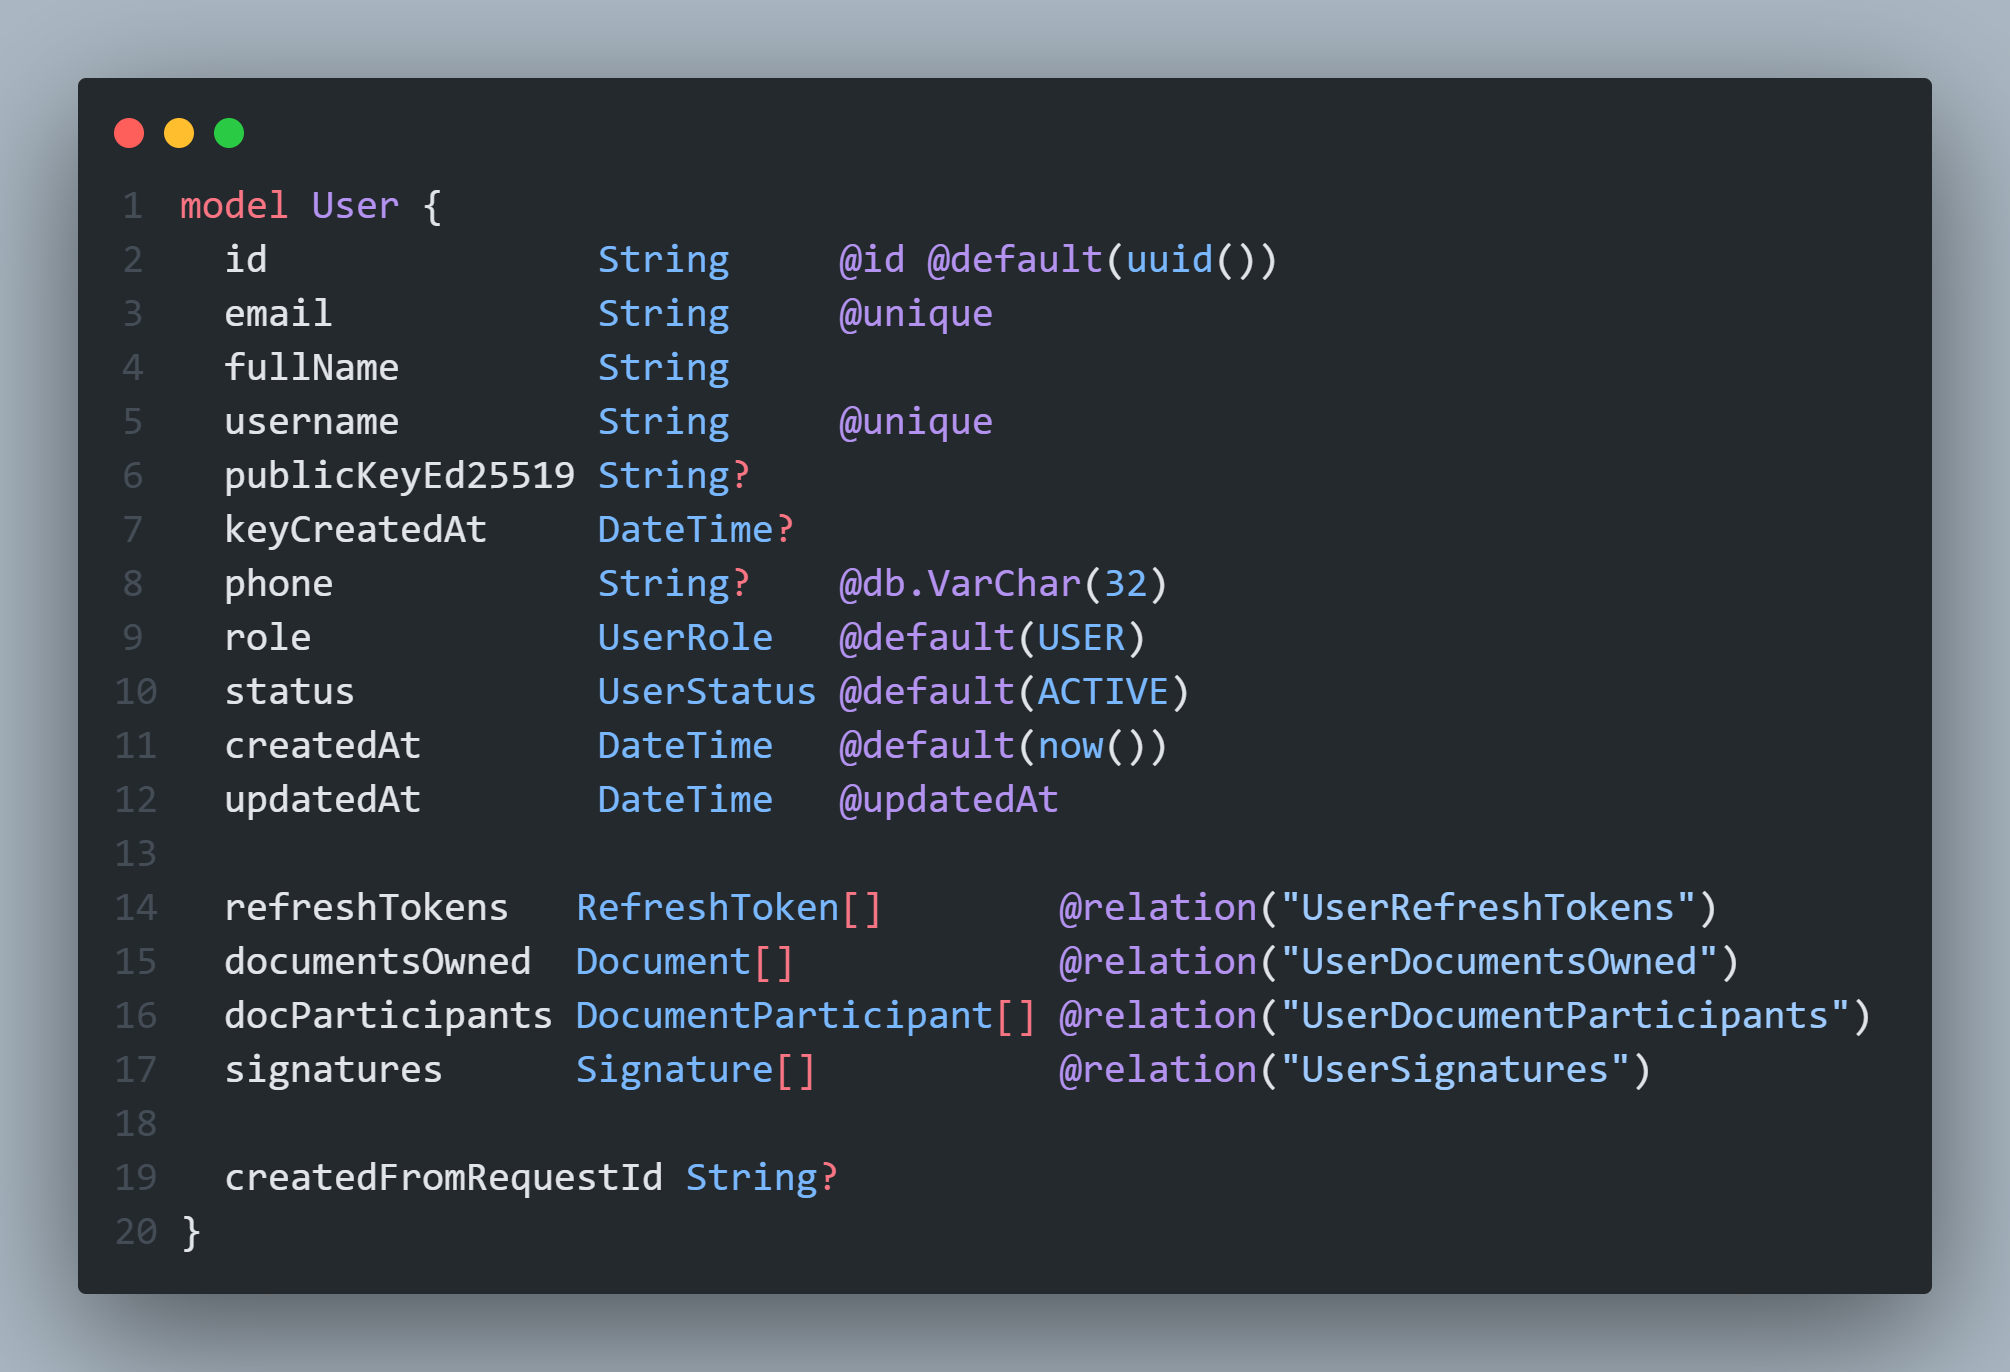
\includegraphics[width=18cm]{"images/user-db-model.png"}
    \caption{User Database Model}
    \label{user-db-model}
\end{figure}

The use of Prisma Client enables type-safe queries and simplifies operations like migrations, seeding, and testing.

\subsection{Security Measures}
The architecture incorporates several security mechanisms. Authentication challenges are valid only for five minutes and become invalid once used. Refresh tokens are stored in secure cookies to reduce exposure. The use of Ed25519 ensures modern cryptographic security, while SHA-256 guarantees the integrity of documents. Finally, file validation ensures that only PDF documents are accepted.

\subsection{Authentication and Tokens}
Authentication in the system is fully passwordless and relies on public/private key pairs. Users prove their identity by signing challenges provided by the server. Successful verification grants them access tokens and refresh tokens in the form of JWTs.

Access tokens are short-lived and returned in the response body, while refresh tokens are long-lived and stored securely in HTTP-only cookies. Middleware functions such as requireUser and requireAdmin check the validity of tokens and enforce role-based access control.

\subsection{Email Service}
The system integrates Nodemailer as an email delivery mechanism configured with SMTP credentials for the project’s domain. Emails are used in two important contexts. First, during registration, users receive a six-digit OTP code for email validation. Second, during document workflows, participants receive notifications when they are asked to review and sign a document, and again when the document has been finalized (Figure \ref{email-sending}).

\begin{figure}[H]
    \centering
    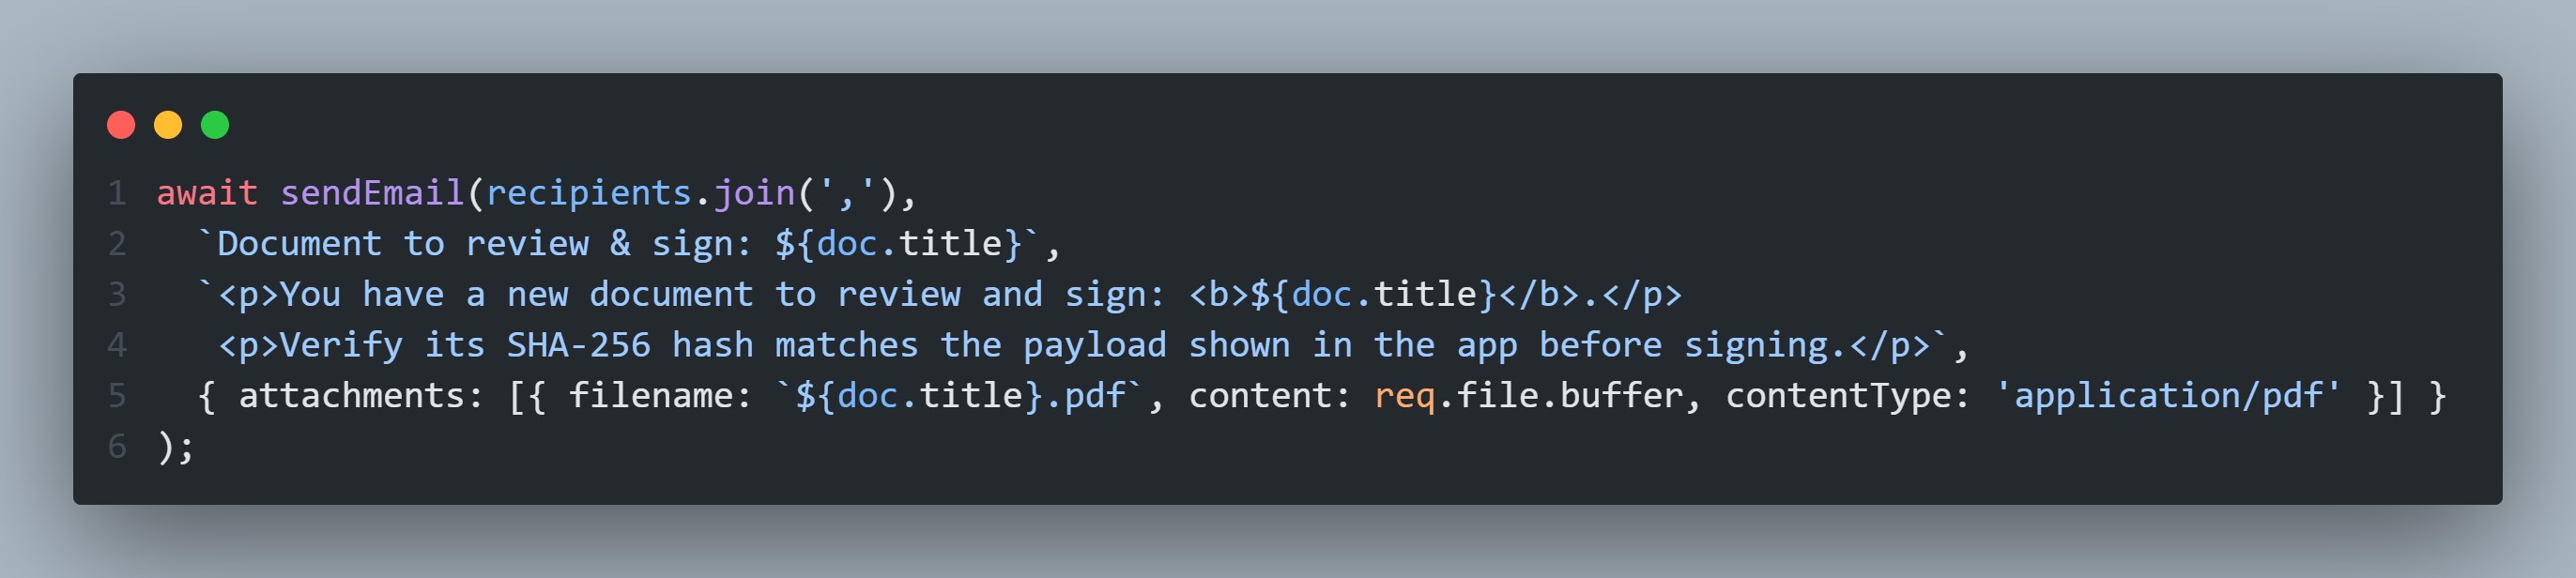
\includegraphics[width=18cm]{"images/email-sending.png"}
    \caption{Email Sending Mechanism}
    \label{email-sending}
\end{figure}

\subsection{Cryptographic Module}
Security of authentication and documents is achieved with the Ed25519 digital signature scheme, implemented via the @noble/ed25519 library (Figure \ref{keygen}). 

\begin{figure}[H]
    \centering
    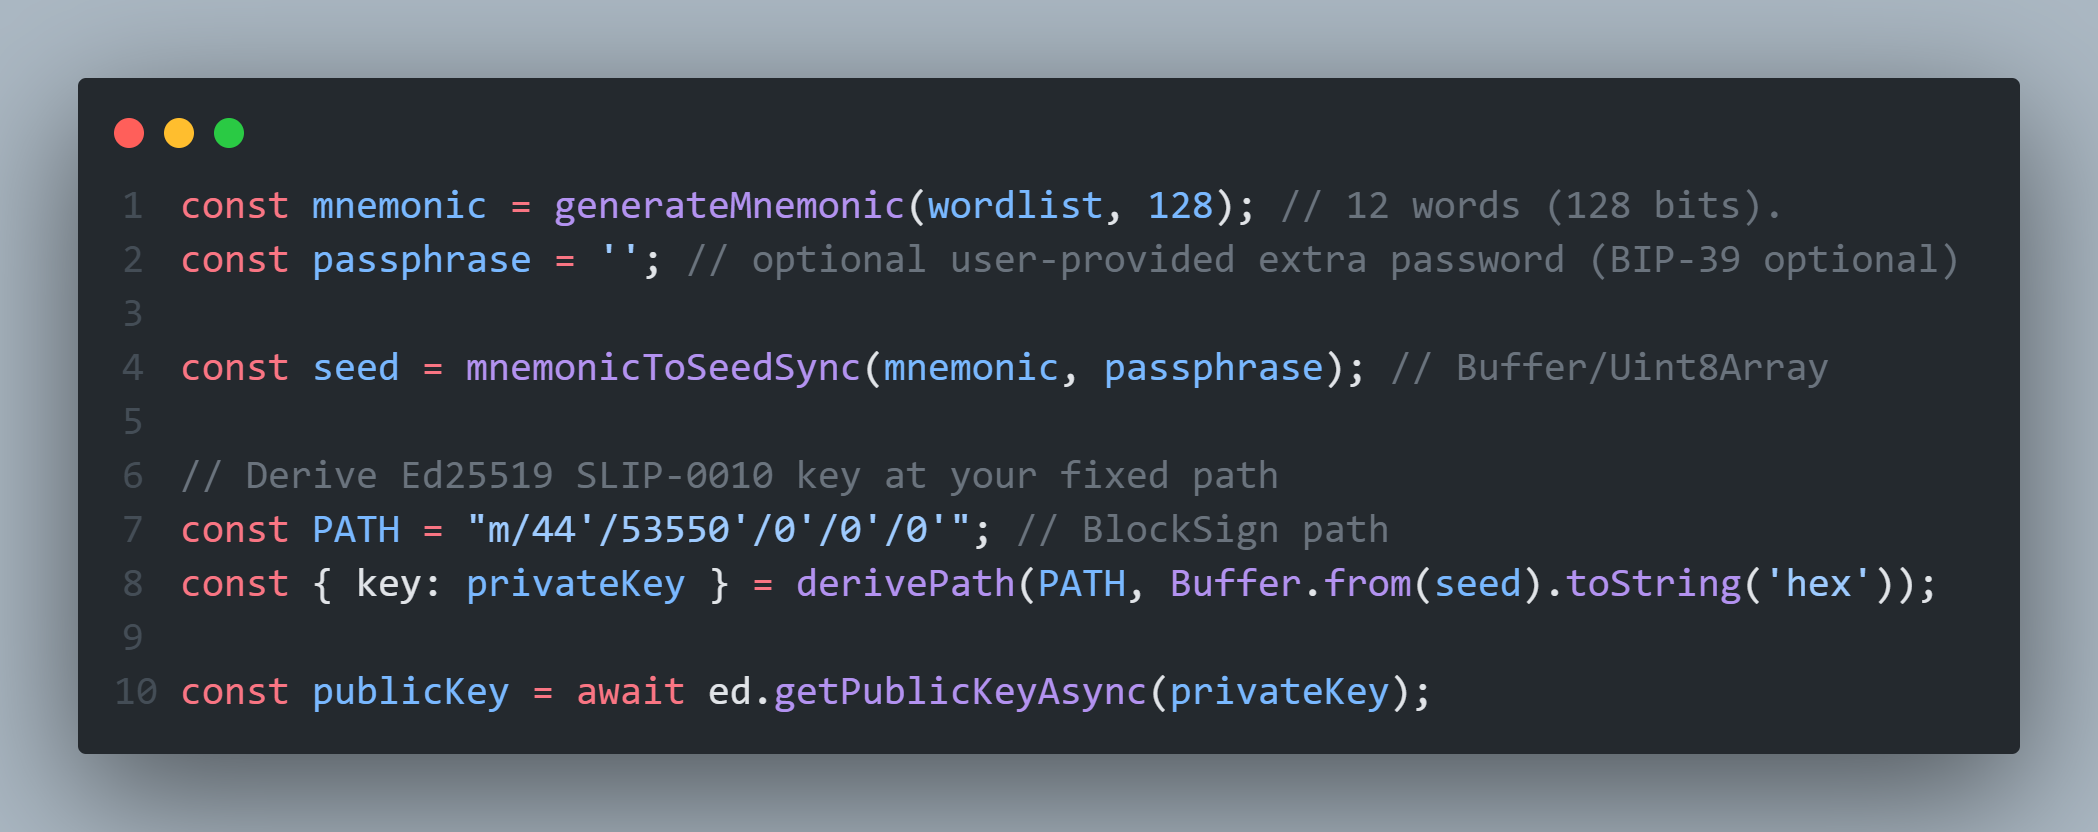
\includegraphics[width=18cm]{"images/keygen.png"}
    \caption{Key Pairs Generation Mechanism}
    \label{keygen}
\end{figure}

A dedicated crypto utility handles key pair generation, signing, and verification of messages. In addition, SHA-256 is used for hashing documents, ensuring their integrity before they are accepted or signed.

\subsection{Document Workflow}
The MVP implementation of the document signing process follows a well-defined lifecycle. When a user creates a document, they upload the file, calculate its SHA-256 hash, and sign a canonical payload. The payload and initial signature are stored in the database.

Participants selected by the creator receive an email with the PDF attached and the corresponding hash. Each participant is expected to calculate the hash independently, compare it with the payload, and if it matches, sign the document (Figure \ref{payload-signature}). 

\begin{figure}[H]
    \centering
    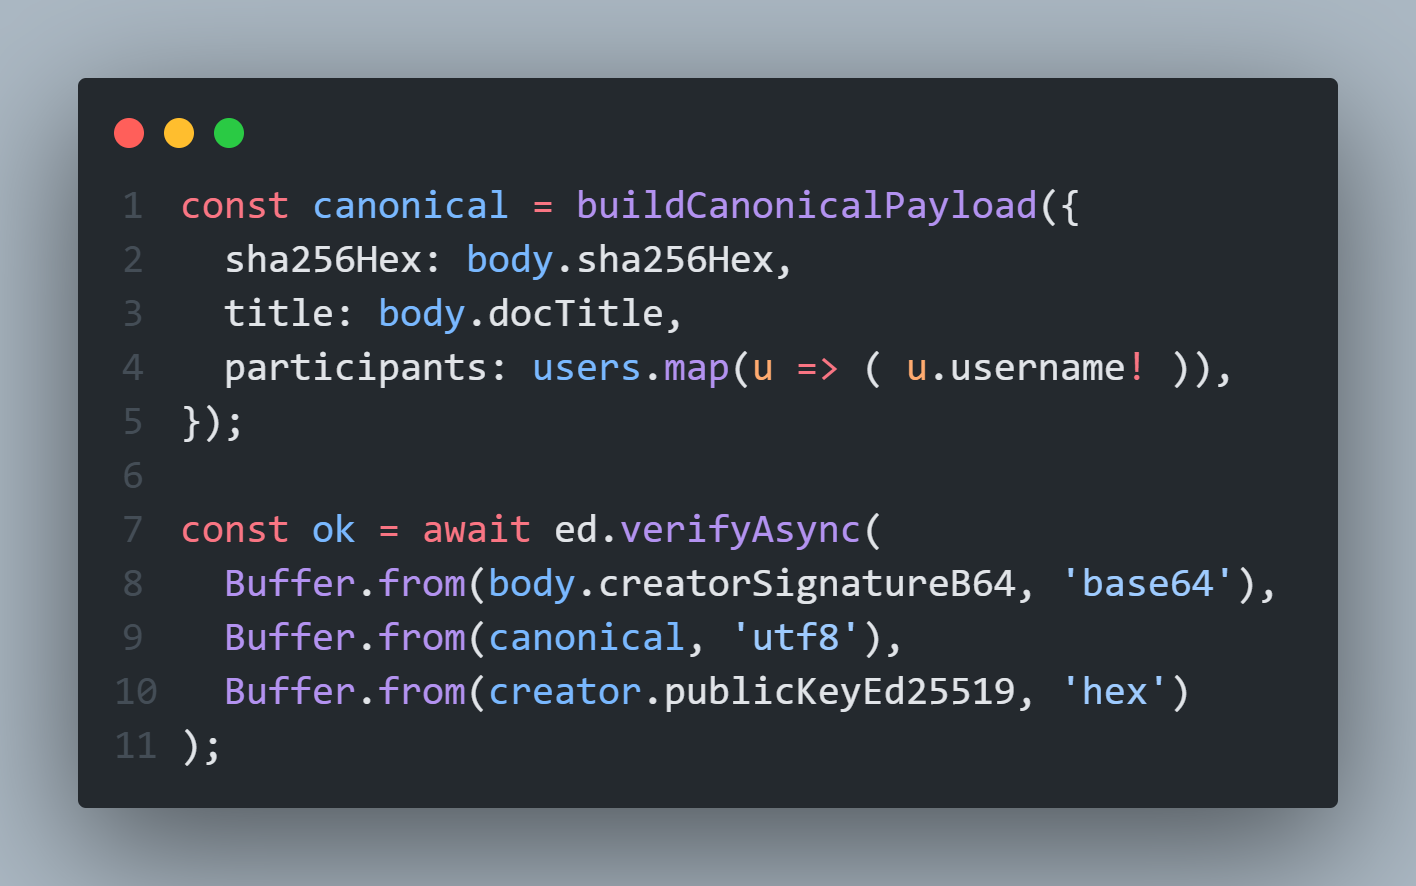
\includegraphics[width=18cm]{"images/payload-signature.png"}
    \caption{Build Paylaod and Verify Signature}
    \label{payload-signature}
\end{figure}

Their signatures are then added to the database. Once all required signatures are collected, the document status changes to signed, and a notification is sent to all involved parties.

\subsection{Extensibility}
The modular design of the back-end makes it adaptable to future improvements. Currently, documents are distributed as email attachments, but the system is ready for integration with external storage providers such as AWS S3. The ChainAnchor entity in the future versions of database will anticipate the anchoring of finalized document hashes on blockchain networks. Similarly, while usernames are currently used to tag participants, the design leaves room for later integration with decentralized identity systems.

\section{Front-end UI}
The front-end of the BlockSign system represents a modern, secure, and user-centric web application built using cutting-edge technologies. The implementation emphasizes client-side security, responsive design, and intuitive user experience while maintaining the highest standards of cryptographic security.

\subsection{Frontend Architecture}
The front-end is built using Next.js 14 with React.js as the core framework, leveraging TypeScript for type safety and enhanced developer experience. The application utilizes Tailwind CSS for styling, providing a consistent and responsive design system across all components (Figure \ref{frontend-stack}).

\begin{figure}[H]
    \centering
    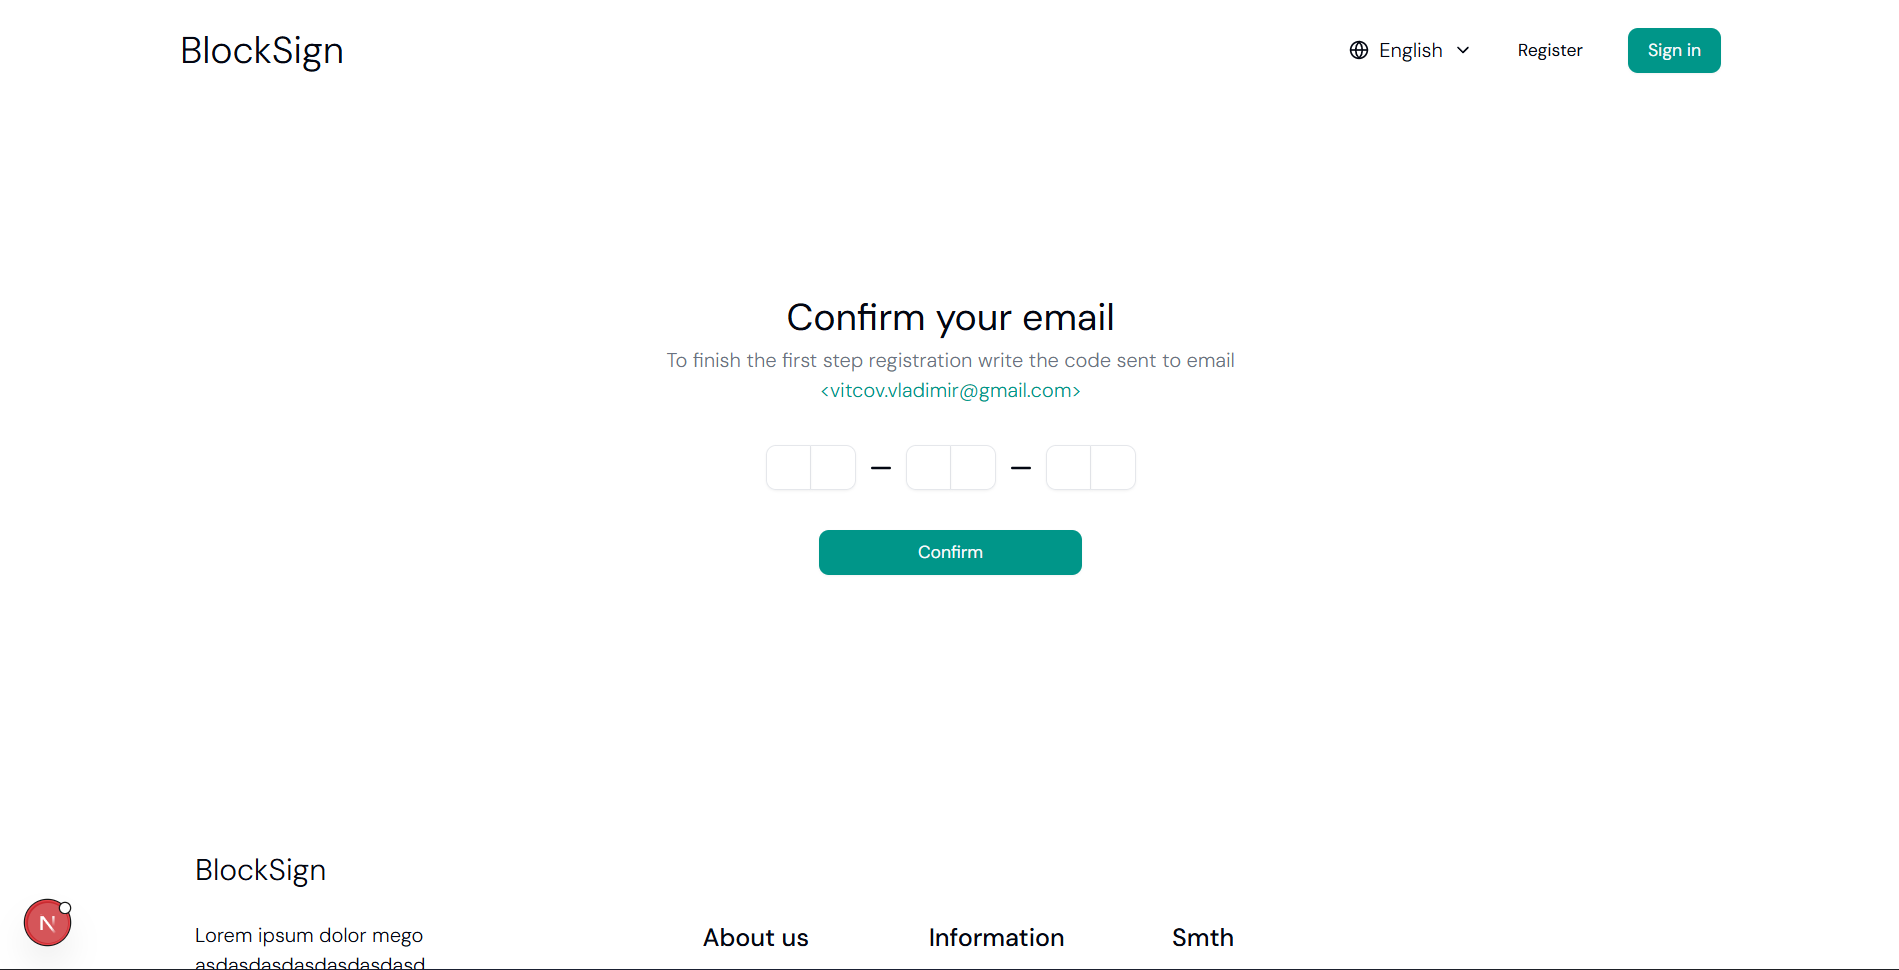
\includegraphics[width=18cm]{"images/siteUI/code.png"}
    \caption{Frontend Technology Stack Implementation}
    \label{frontend-stack}
\end{figure}

The architecture follows a modular component-based approach with clear separation of concerns:

\begin{itemize}
    \item \textbf{Presentation Layer}: React components with Tailwind CSS styling
    \item \textbf{State Management}: React Context API for global state management
    \item \textbf{Security Layer}: Client-side cryptographic operations and secure key management
    \item \textbf{Communication Layer}: HTTP clients for API communication with the backend
    \item \textbf{Internationalization}: Multi-language support with i18next
\end{itemize}

The front-end implementation prioritizes client-side security, ensuring that sensitive information such as private keys and mnemonic phrases never leave the user's browser. This approach aligns with the zero-trust security model and provides users with complete control over their cryptographic materials.

\subsection{Landing Page and User Onboarding}
The landing page serves as the primary entry point for users, featuring a clean and professional design that communicates the platform's value proposition effectively. The page is structured to provide comprehensive information about BlockSign's capabilities while maintaining an elegant and accessible design.

\subsubsection{Landing Page Design and Layout}
The landing page follows modern web design principles with a focus on clarity, accessibility, and conversion optimization. The page is divided into several key sections that progressively introduce users to the platform's features and benefits.

The header section features the BlockSign logo and navigation menu, providing immediate access to registration and login functionality. The hero section contains a compelling value proposition with clear call-to-action buttons that guide users toward registration or learning more about the platform.

The design emphasizes trust and security through the use of professional typography, consistent color schemes, and carefully selected imagery that reinforces the platform's reliability and sophistication.

\subsubsection{Feature Presentation}
The landing page includes dedicated sections that highlight BlockSign's key features:

\begin{itemize}
    \item \textbf{Passwordless Authentication}: Emphasis on modern security through cryptographic keys
    \item \textbf{Document Integrity}: Explanation of cryptographic verification and tamper-proof signatures
    \item \textbf{Multi-party Signing}: Collaborative document workflows with multiple participants
    \item \textbf{Regulatory Compliance}: Adherence to international digital signature standards
    \item \textbf{User Privacy}: Client-side cryptography and zero-trust architecture
\end{itemize}

\subsubsection{Educational Content}
The landing page serves an educational purpose by explaining digital signature concepts to users who may be unfamiliar with cryptographic authentication. This includes simplified explanations of:

\begin{itemize}
    \item How digital signatures work and why they're more secure than traditional methods
    \item The benefits of passwordless authentication using mnemonic phrases
    \item Document integrity verification and tamper detection
    \item Legal validity and compliance aspects of digital signatures
\end{itemize}

\subsubsection{Trust Indicators}
The page incorporates various trust indicators to build user confidence:

\begin{itemize}
    \item Security certifications and compliance badges
    \item Transparent explanation of the platform's security architecture
    \item Clear privacy policy and data handling practices
    \item Educational resources about digital signature technology
\end{itemize}

The user onboarding process is designed to be intuitive and secure, guiding users through each step of the registration and setup process with clear instructions and visual feedback. Progressive disclosure techniques are used to avoid overwhelming new users while ensuring they understand the security implications of their actions.

\subsection{Registration Flow and User Identity}
The registration process implements a multi-step verification system that ensures user authenticity while maintaining privacy. The flow begins with basic user information collection and email verification through OTP (One-Time Password) codes.

Users receive an email containing a six-digit verification code that must be entered to proceed with the registration (Figure \ref{registration-email}).

\begin{figure}[H]
    \centering
    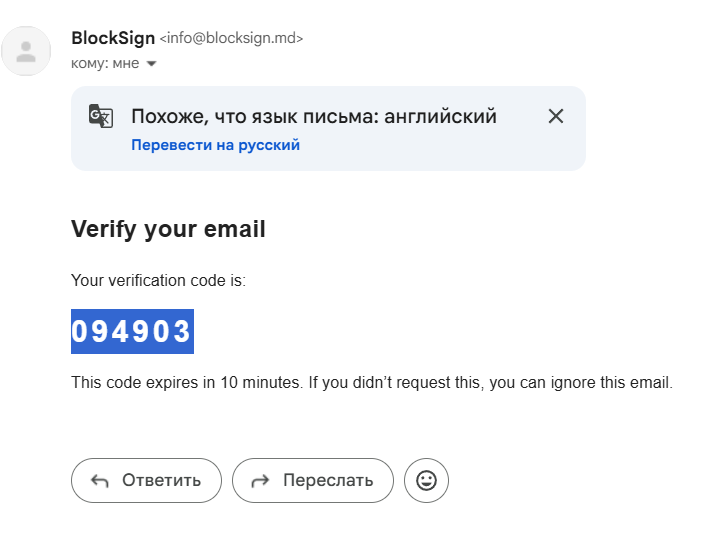
\includegraphics[width=18cm]{"images/siteUI/codeMail.png"}
    \caption{Email Verification Code}
    \label{registration-email}
\end{figure}

The registration form captures essential user information including full name, email, phone number, and IDNP (personal identification number) for identity verification purposes (Figure \ref{registration-form}).

\begin{figure}[H]
    \centering
    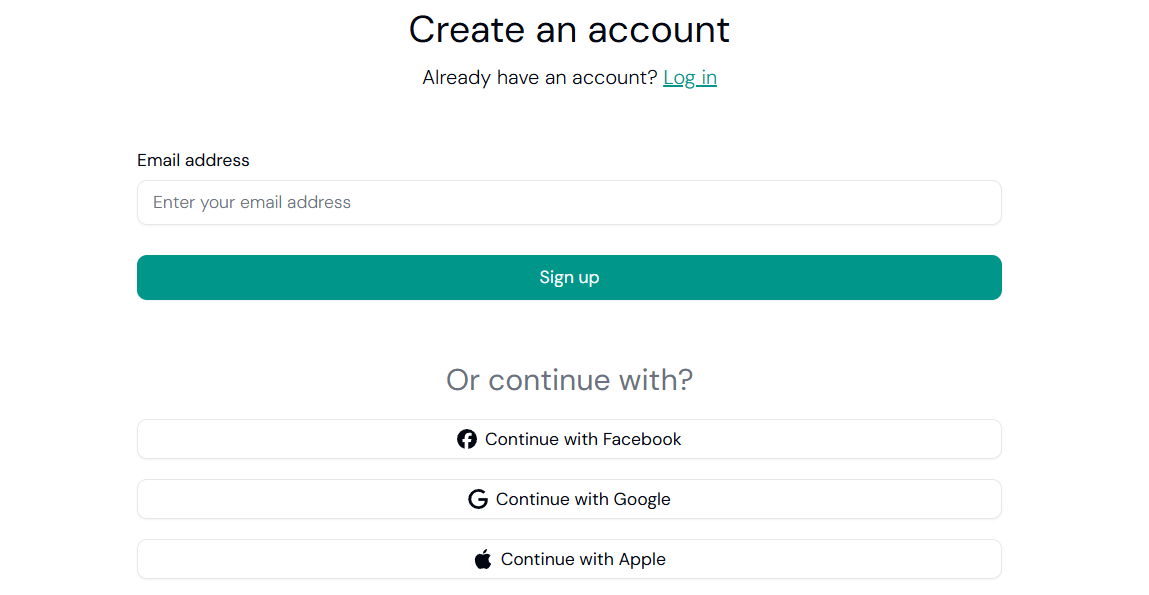
\includegraphics[width=18cm]{"images/siteUI/register.png"}
    \caption{User Registration Form}
    \label{registration-form}
\end{figure}

Upon successful submission, users see a confirmation page indicating that their registration request has been submitted for administrative review (Figure \ref{registration-success}).

\begin{figure}[H]
    \centering
    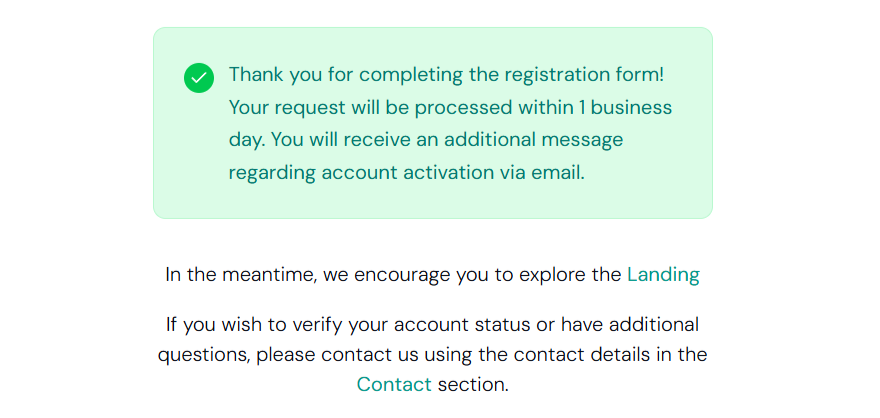
\includegraphics[width=18cm]{"images/siteUI/thankYou.png"}
    \caption{Registration Success Confirmation}
    \label{registration-success}
\end{figure}

Once the administrator approves the registration request, users receive a notification email to complete their account setup.

\subsection{Authentication System and Security Features}
The authentication system implements a passwordless approach using cryptographic key pairs and mnemonic phrases. This section details the user interface components that facilitate secure authentication while maintaining usability.

\subsubsection{Mnemonic-Based Authentication}
After registration approval, users are guided through a secure key generation process. The system generates a 12-word mnemonic phrase that serves as the master key for the user's cryptographic identity. This approach ensures that users maintain complete control over their authentication credentials without relying on traditional password-based systems.

The mnemonic phrase generation interface provides clear instructions for users to securely store their recovery phrase (Figure \ref{mnemonic-phrase}). The interface emphasizes the importance of keeping the phrase secure and warns users about the consequences of losing access to it.

Users are presented with additional security options, including the ability to set up a PIN for convenient access while maintaining the security of the mnemonic phrase (Figure \ref{security-method}). This dual-layer approach balances security with user convenience.

\subsubsection{PIN-Based Quick Access}
For enhanced user experience, the system offers an optional PIN-based authentication method that allows users to access their accounts without entering the full mnemonic phrase for routine operations (Figure \ref{pin-for-site}). The PIN is stored locally and encrypted using the user's public key, ensuring that it cannot be used without the corresponding private key.

\subsubsection{Secure Login Interface}
The login interface supports both mnemonic phrase authentication and PIN-based access. Users can choose their preferred authentication method based on their security preferences and usage patterns (Figure \ref{mnemonic-login}).

\begin{figure}[H]
    \centering
    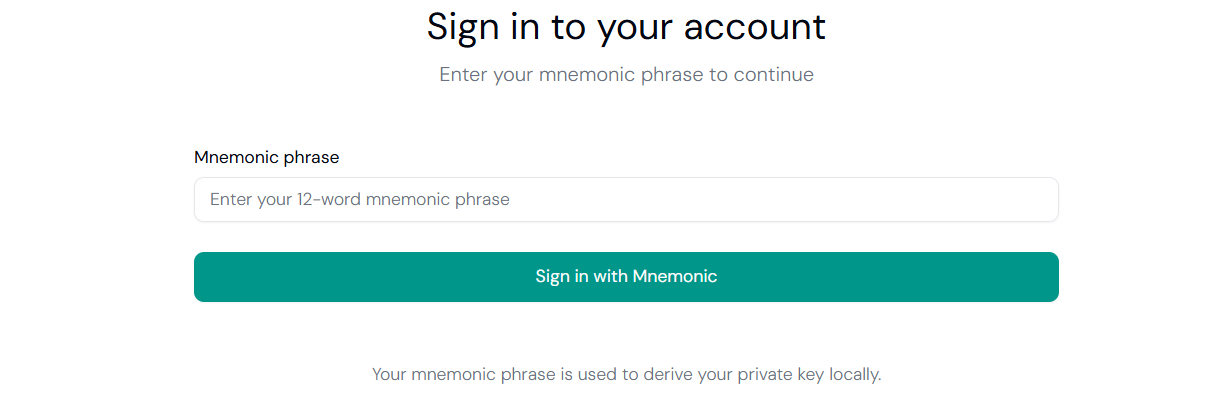
\includegraphics[width=18cm]{"images/siteUI/mnemonicLogin.png"}
    \caption{Mnemonic-Based Login Interface}
    \label{mnemonic-login}
\end{figure}

The interface provides clear feedback during the authentication process and includes security features such as automatic session timeout and secure token management.

\subsection{User role specified UI}
The authorized user is represented by the possibility to view his account info in the header as well as having acess to the authorized only pages (Figure \ref{header-account-user}).

\begin{figure}[H]
    \centering
    
\includegraphics[width=18cm]{"images/siteUI/headerAccountUser.png"}
    \caption{Header Account User}
    \label{header-account-user}
\end{figure}

Also there is some difference for the admin header, it has additional button to navigate to the admin console (Figure \ref{header-account-admin}).

\begin{figure}[H]
    \centering
    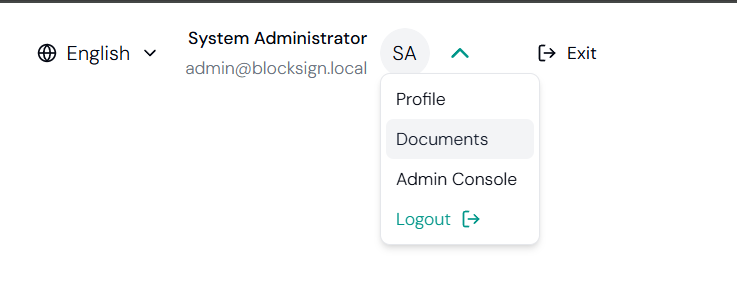
\includegraphics[width=18cm]{"images/siteUI/headerAccountAdmin.png"}
    \caption{Header Account Admin}
    \label{header-account-admin}
\end{figure}

Navigating to the admin console will lead to the following page (Figure \ref{admin-console}):

\begin{figure}[H]
    \centering
    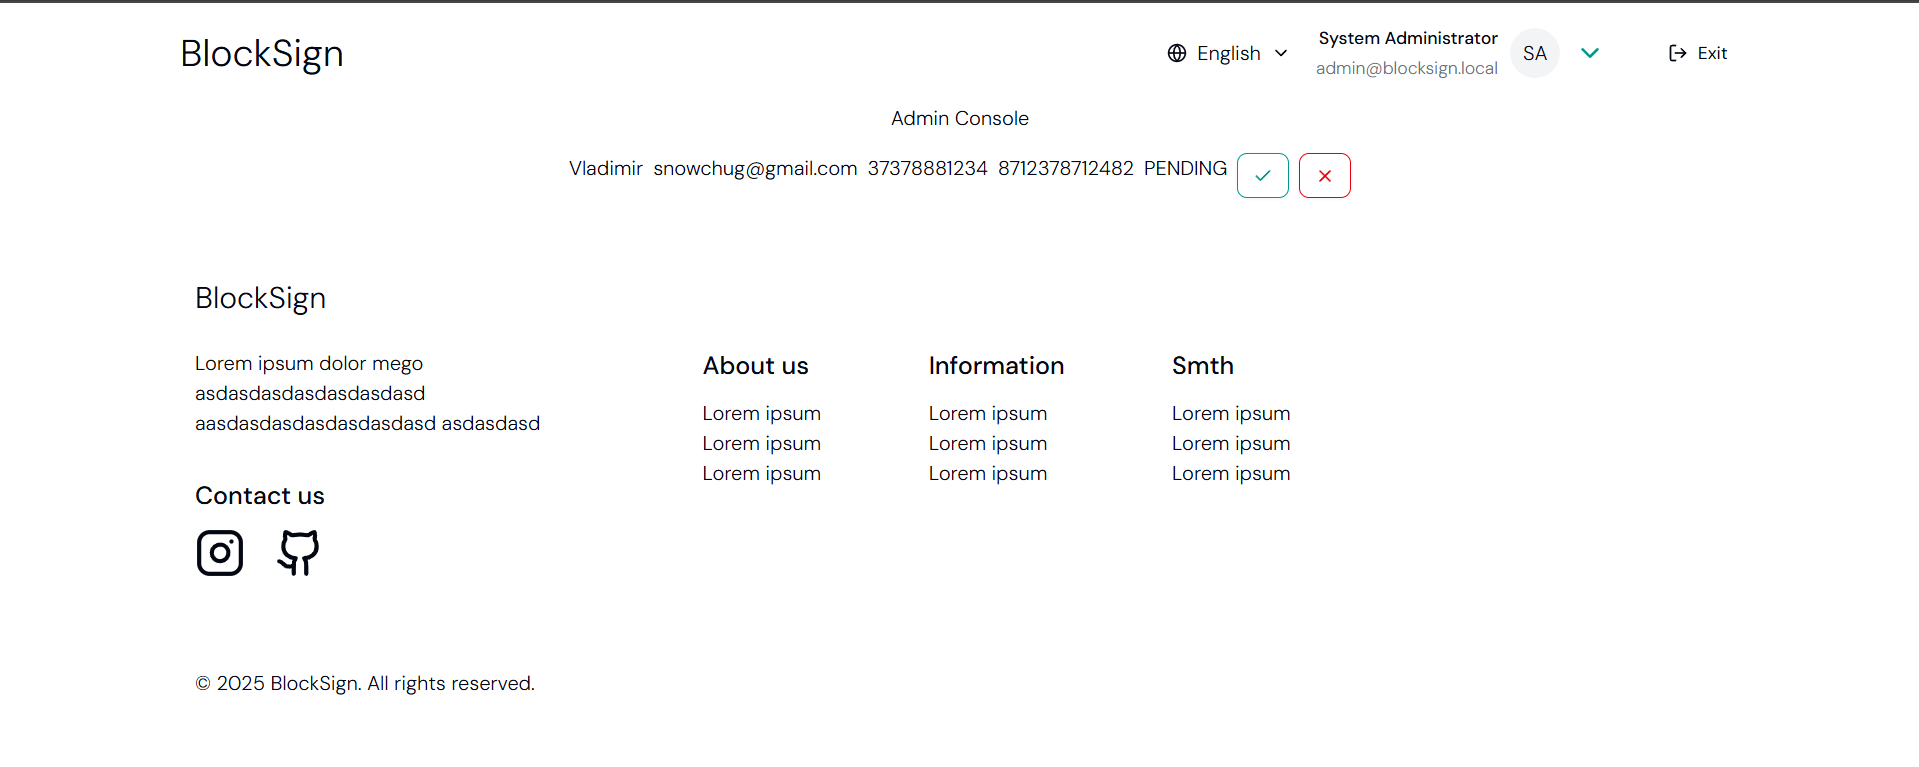
\includegraphics[width=18cm]{"images/siteUI/adminConsole.png"}
    \caption{Admin Console}
    \label{admin-console}
\end{figure}

On this page the admin can confirm or reject the registration requests. The requests are listed in the table with the following information:

\begin{itemize}
    \item Full Name
    \item Email
    \item Phone
    \item idnp
    \item Action
\end{itemize}

If there are no requests, the admin will see the following page (Figure \ref{admin-console-empty}):

\begin{figure}[H]
    \centering
    
\includegraphics[width=18cm]{"images/siteUI/adminConsoleNoRequests.png"}
    \caption{Admin Console Empty}
    \label{admin-console-empty}
\end{figure}

\subsection{Additional registration steps}

Then an email with the finish of the registration process is sent to the user (Figure \ref{finish-registration-mail}).

\begin{figure}[H]
    \centering
    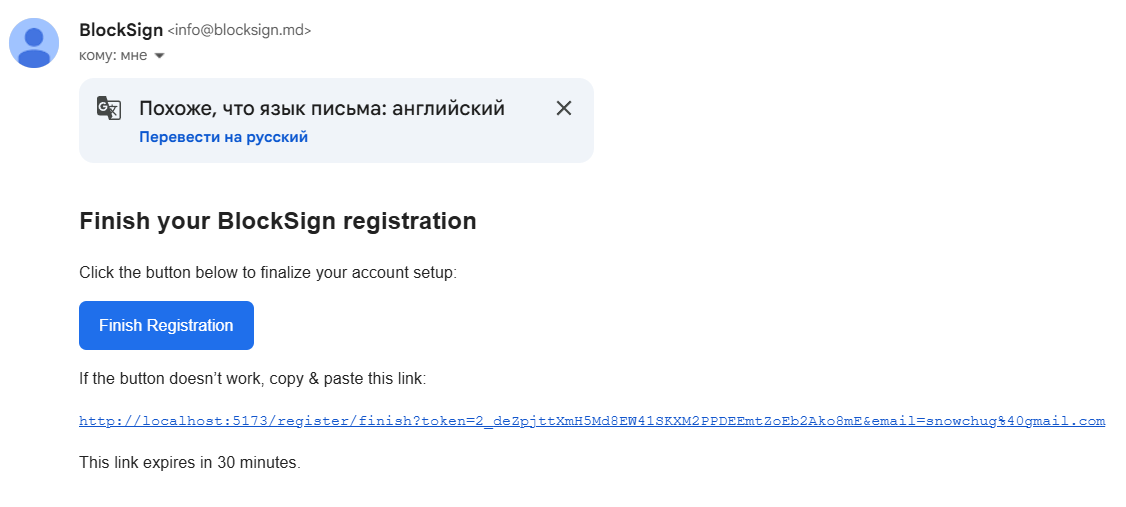
\includegraphics[width=18cm]{"images/siteUI/finishRegMail.png"}
    \caption{Finish Registration Mail}
    \label{finish-registration-mail}
\end{figure}

Clicking the button or link will lead to the following page (Figure \ref{mnemonic-phrase}):

\begin{figure}[H]
    \centering
    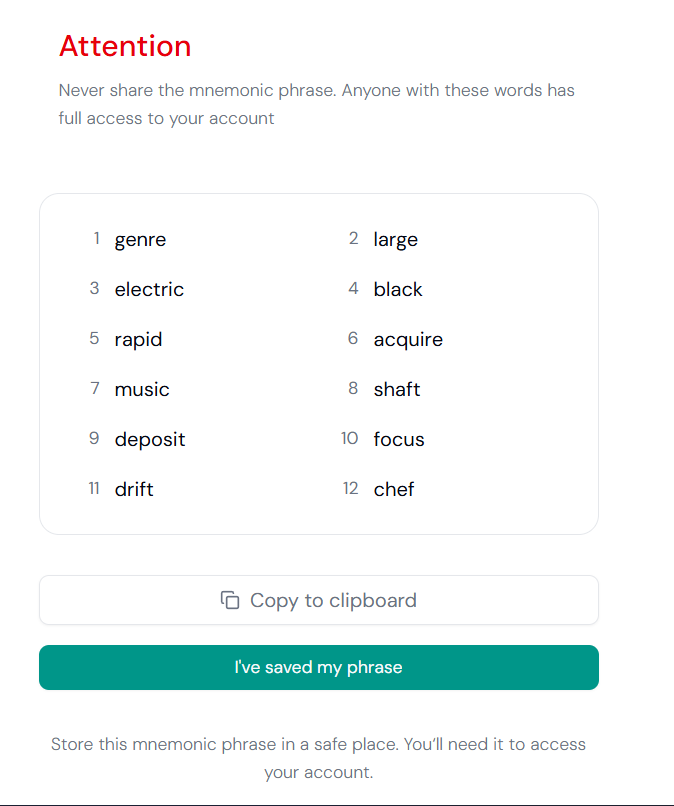
\includegraphics[width=18cm]{"images/siteUI/mnemonicPhrase.png"}
    \caption{Mnemonic Phrase}
    \label{mnemonic-phrase}
\end{figure}

Here the user can see his mnemonic phrase and store it in a secure way (Figure \ref{mnemonic-phrase}). The phrase is generated on each refresh, but is valid only after clicking the button continue otherwise it is not valid anywhere. Then the user can choose to set a pin or remain only with mnemonic phrase (Figure \ref{security-method}).

\begin{figure}[H]
    \centering
    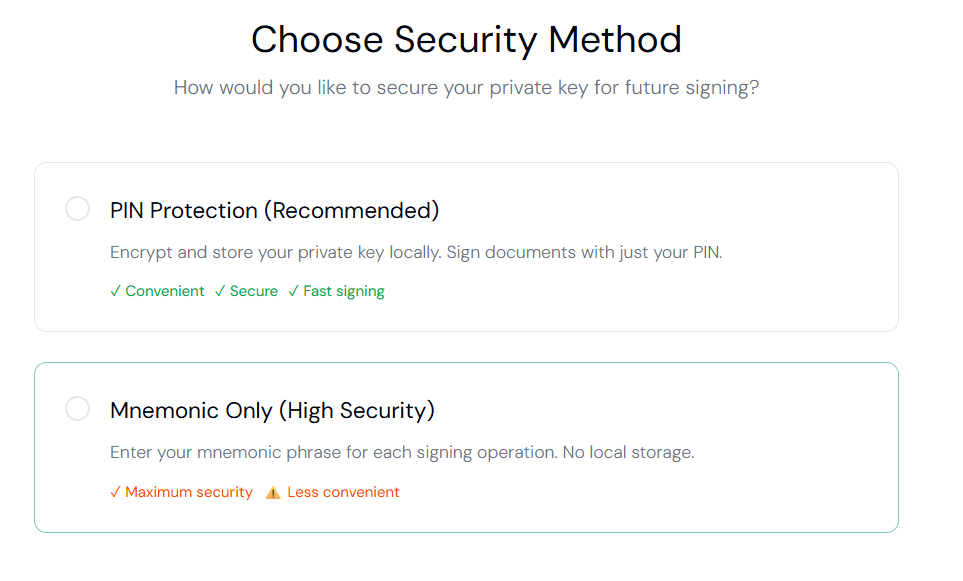
\includegraphics[width=18cm]{"images/siteUI/securityMethod.png"}
    \caption{Security Method Selection}
    \label{security-method}
\end{figure}

Then the user can set a pin for the site (Figure \ref{pin-for-site}). The pin is a shorter way to access the account and site functionality to avoid using the mnemonic phrase every time. 

\begin{figure}[H]
    \centering
    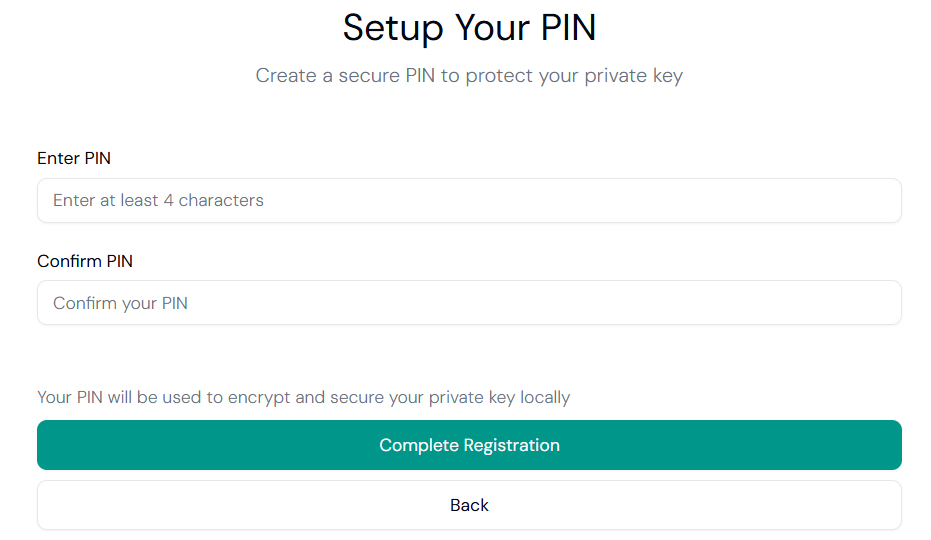
\includegraphics[width=18cm]{"images/siteUI/pinForSite.png"}
    \caption{PIN Setup for Convenient Access}
    \label{pin-for-site}
\end{figure}

\subsection{Document Management Interface}
The document management system provides users with comprehensive tools for creating, signing, and managing digital documents. The interface is designed to streamline the document workflow while maintaining the highest security standards.

\subsubsection{Dashboard and Navigation}
Once authenticated, users are presented with a clean and intuitive dashboard that provides access to all document-related functionality. The dashboard displays recent document activity, pending signature requests, and quick access to document creation tools (Figure \ref{logged-in-dashboard}).

\begin{figure}[H]
    \centering
    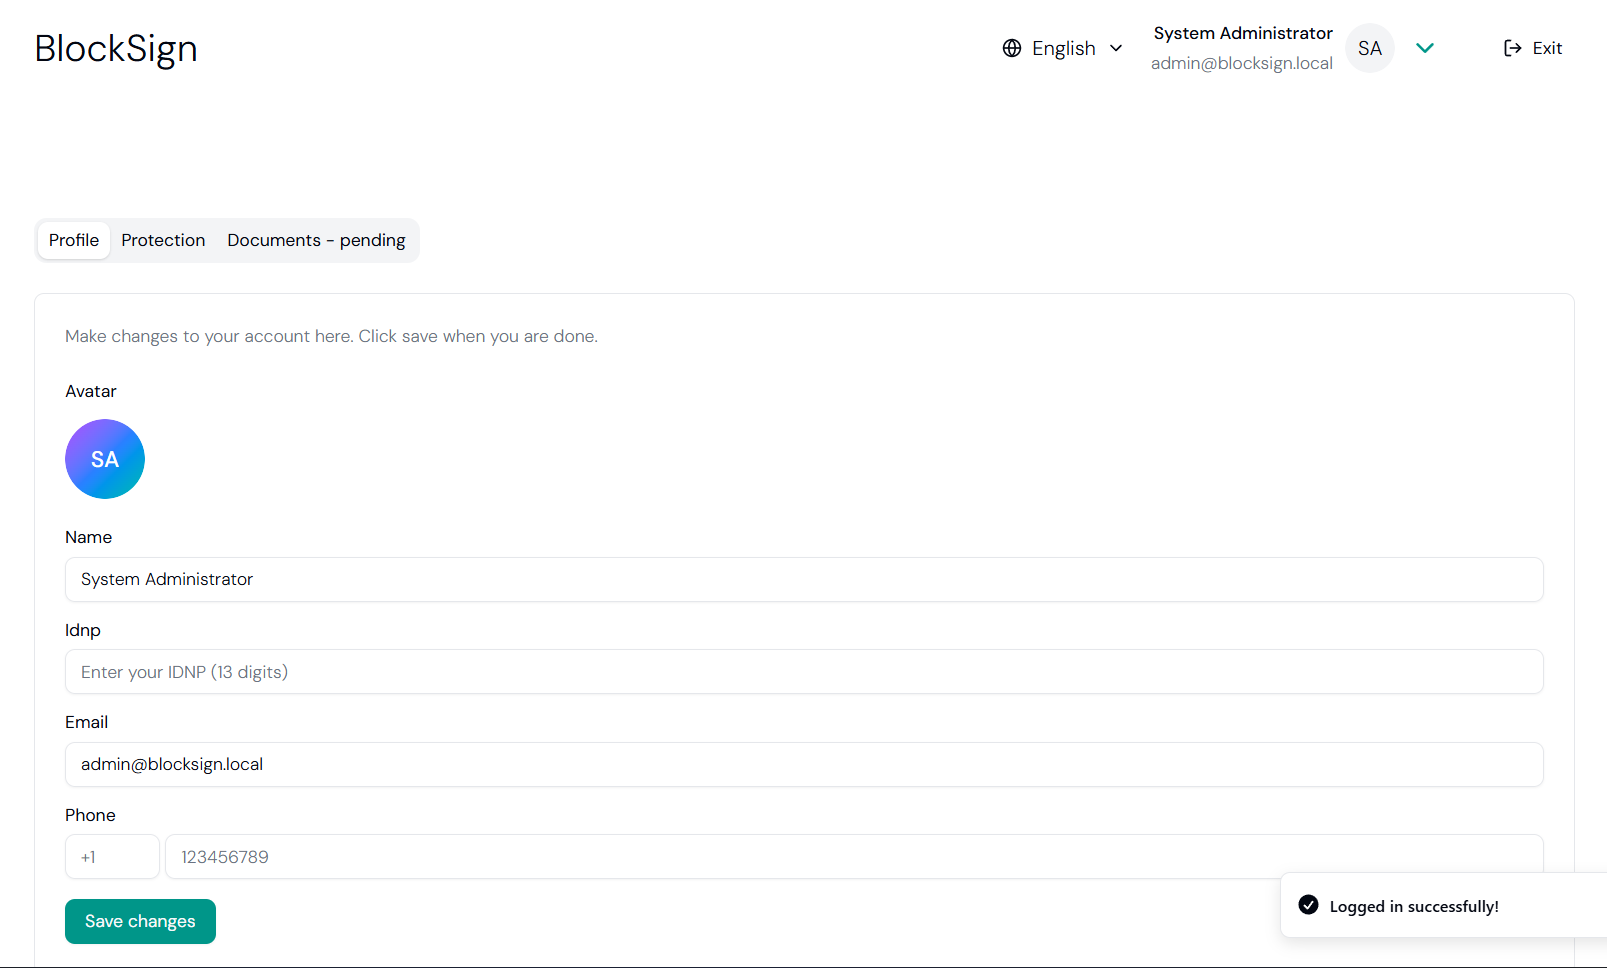
\includegraphics[width=18cm]{"images/siteUI/logedIn.png"}
    \caption{User Dashboard After Login}
    \label{logged-in-dashboard}
\end{figure}

The navigation system is designed to be intuitive, with clear visual indicators for different user roles and permissions. Authorized users can easily access their document library, create new documents, and manage their account settings.

\subsubsection{Document Creation and Upload}
The document creation process guides users through uploading PDF files and configuring signature requirements. The interface includes drag-and-drop functionality for easy file upload, along with validation to ensure only supported file formats are accepted.

Users can specify multiple participants for document signing, with each participant receiving notification emails containing the document and instructions for the signing process. The system automatically generates cryptographic hashes for document integrity verification.

\subsubsection{Document Signing Workflow}
The signing interface provides a secure environment for users to review and sign documents. Before signing, users can verify the document's integrity by comparing cryptographic hashes. The interface clearly displays document metadata, participant information, and signing status.

The signing process requires users to authenticate using their mnemonic phrase or PIN, ensuring that only authorized individuals can create valid signatures. Real-time feedback is provided throughout the signing process, including confirmation of successful signature creation and verification.

\subsubsection{Document History and Verification}
Users can access a comprehensive history of all documents they have created or signed. The interface provides detailed information about each document, including creation date, participants, signature status, and verification results.

The verification interface allows users to upload documents and verify their authenticity by checking cryptographic signatures and document integrity. This feature is available to both registered users and anonymous visitors, promoting transparency and trust in the digital signature process.

\subsection{Responsive Design and User Experience}
The BlockSign frontend implements a fully responsive design that adapts seamlessly to different screen sizes and devices. The application provides an optimal user experience across desktop computers, tablets, and mobile devices.

\subsubsection{Mobile-First Approach}
The design follows a mobile-first approach, ensuring that the core functionality is accessible and usable on smaller screens. Tailwind CSS breakpoints are used strategically to provide device-specific layouts and component arrangements.

Key responsive features include:
\begin{itemize}
    \item Adaptive navigation menus that collapse on mobile devices
    \item Touch-friendly button sizes and interactive elements
    \item Optimized form layouts for mobile input
    \item Responsive image scaling and document previews
    \item Accessible typography and color contrast ratios
\end{itemize}

\subsubsection{Cross-Browser Compatibility}
The application is tested and optimized for modern web browsers, including Chrome, Firefox, Safari, and Edge. The codebase uses progressive enhancement techniques to ensure functionality across different browser versions while providing enhanced features for newer browsers.

\subsection{Client-Side Security Implementation}
The frontend architecture prioritizes security at every level, implementing multiple layers of protection for user data and cryptographic operations. All sensitive operations are performed client-side to minimize the exposure of private information.

\subsubsection{Cryptographic Key Management}
Private keys and mnemonic phrases are never transmitted to the server. All cryptographic operations, including key generation, signing, and verification, are performed within the user's browser using JavaScript cryptographic libraries.

The system implements secure storage mechanisms for sensitive data:
\begin{itemize}
    \item Mnemonic phrases are stored temporarily in memory during active sessions
    \item PIN codes are encrypted using public keys before local storage
    \item Session tokens are managed securely with automatic expiration
    \item Private keys are derived from mnemonic phrases on-demand
\end{itemize}

\subsubsection{Secure Communication}
All communication between the frontend and backend uses HTTPS encryption. The application implements Content Security Policy (CSP) headers to prevent cross-site scripting attacks and other security vulnerabilities.

API requests are authenticated using JWT tokens with short expiration times, and refresh tokens are stored in secure HTTP-only cookies to prevent JavaScript-based attacks.

\subsection{Internationalization and Localization}
The application supports multiple languages to serve a diverse user base. The internationalization system uses i18next for dynamic language switching and locale-specific formatting.

\subsubsection{Multi-Language Support}
Currently supported languages include:
\begin{itemize}
    \item English (default)
    \item Romanian
    \item Russian
\end{itemize}

The language selection interface allows users to switch between supported languages dynamically, with all text content, error messages, and user interface elements updating accordingly.

\subsubsection{Localization Features}
The localization system handles:
\begin{itemize}
    \item Date and time formatting according to locale preferences
    \item Number formatting and currency display
    \item Text direction support for future RTL language integration
    \item Culturally appropriate messaging and terminology
\end{itemize}

\subsection{Feature Accessibility by User Role}

The BlockSign platform implements a role-based access control system that provides different levels of functionality based on user authentication status and administrative privileges.

\subsubsection{Public Features (Unauthorized Users)}
Unauthorized users have access to essential platform information and basic functionality without requiring registration:

\begin{itemize}
    \item \textbf{Platform Information}: Access to landing page content, feature descriptions, and educational materials about digital signatures
    \item \textbf{User Registration}: Complete registration process including email verification and account request submission
    \item \textbf{Document Verification}: Upload and verify the authenticity of signed documents using cryptographic verification
    \item \textbf{Multi-language Support}: Switch between supported languages for better accessibility
\end{itemize}

\subsubsection{Authenticated User Features}
Registered and verified users gain access to comprehensive document management capabilities:

\begin{itemize}
    \item \textbf{Document Creation}: Upload PDF documents and initiate signature workflows with multiple participants
    \item \textbf{Digital Signing}: Sign documents using cryptographic keys with mnemonic phrase or PIN authentication
    \item \textbf{Document History}: View complete history of created and signed documents with detailed metadata
    \item \textbf{Signature Management}: Track signature status for multi-party documents and receive notifications
    \item \textbf{Account Management}: Update profile information, manage security settings, and configure notification preferences
    \item \textbf{Participant Coordination}: Invite other users to sign documents and manage participant workflows
    \item \textbf{Document Verification}: Verify signatures on received documents and check document integrity
    \item \textbf{Secure Storage}: Access encrypted document metadata and signature records
\end{itemize}

\subsection{Technology Integration and Performance}
The frontend implementation leverages modern web technologies to provide optimal performance and user experience across different devices and network conditions.

\subsubsection{Performance Optimization}
Key performance features include:
\begin{itemize}
    \item \textbf{Code Splitting}: Dynamic imports and lazy loading for reduced initial bundle size
    \item \textbf{Image Optimization}: Automatic image compression and format selection for faster loading
    \item \textbf{Caching Strategy}: Strategic use of browser caching for static assets and API responses
    \item \textbf{Progressive Loading}: Incremental content loading to improve perceived performance
\end{itemize}